\chapter{Python}
Python is very concise and good for scripting.
It is the most used general purpose language, and there are many nice Machine Learning libraries.

Its two key aspects are that it is \textbf{interpreted} ($\neq compiled$) and \textbf{dynamically typed}.

Aside from these two main aspects, we can discuss a few others:\\
even if not as much as Java, it's \textbf{object} oriented;
Python supports both \textbf{imperative} and \textbf{functional} paradigms.\\
Python \textbf{Iterators} can be associated with \texttt{List}s in Haskell and \texttt{Stream}s in Java.
Other Python features are:
\begin{itemize}
   \item Powerful subscripting (slicing)
   \item Higher-order functions
   \item Flexible signatures, which compensate the lack of complex polymorphism
   \item Java-like exceptions
   \item (bad) Multithreading support
\end{itemize}

Let's discuss how Python addresses \textbf{typing}:
\begin{enumerate}
   \item Variables come into existence when first assigned to
   \item Variables are \textit{not} \textit{typed}, but \underline{Values are}!
   \item A variable can refer to an object of any type
   \item It is \textbf{Strongly typed} in the sense that the \textit{value type} does not change in unexpected ways
   \item It is \textbf{Type-safe} since no conversion or operation can be applied to values of the \textbf{wrong} type
\end{enumerate}


Variables come into existence when first assigned and a variable can refer to an object of any type,
besides all types are (almost) treated the same way.
Even if this allows for concise syntax and intuitive code writing, it also implies a main drawback: \underline{\textbf{type errors} are only caught at \textit{runtime}}.

\section{Some Python aspects}
\begin{itemize}
   \item \textbf{Indentation} matters, and is used opposed to brackets \texttt{\{\}}
   \item A variable is created when some value is assigned to it
   \item Assignments in Python \textbf{do not} create a copy
   \note{Even for \texttt{Integer}s!}
   \item Objects are deleted by the garbage collector once they become unreachable
   \begin{itemize}
      \item \texttt{CPython} uses \textit{reference counting} along with \texttt{Mark \& Sweep} for garbage collection
   \end{itemize}
   \item 
   \end{itemize}

\section{Data Types and operators}
\textit{Integers} are \textbf{unbounded},
while \texttt{Float}s are represented with 64 bits.\\
There are no logical symbols, the operators are \texttt{and, or, not}.\\
Strings can be enclosed in \texttt{''}, \texttt{""}, \texttt{""" """},
with the third that allows multiline strings (\textit{cool!}).

\subsection{Sequence types}
\texttt{Tuples}, \texttt{Strings} and \texttt{Lists} are the sequence types in Python, they are \textit{immutable} except for Lists.

They all support \textbf{slicing}, concatenation (\lstinline|+|) and membership (\lstinline|in|).

\textbf{Slicing} returns a subsequence of the original sequence, a \textbf{copy}.
Start copying
at the first index, and stop copying \textit{before} the second index.

\lstset{language=python}
\begin{lstlisting}
   >>> t = (23, 'abc', 4.56, (2,3), 'def')
   >>> t[1:4] # ('abc', 4.56, (2,3))
   >>> t[1:-1] # negative indices ('abc', 4.56, (2,3))
   >>> t[1:-1:2] # optional argument: step ('abc', (2,3))
   >>> t[:2] # no first index: from beginning (23, 'abc')
   >>> t[2:] # no second index: to end (4.56, (2,3), 'def')
   >>> t[:] # no indexes: creates a copy (23, 'abc', 4.56, (2,3), 'def')
\end{lstlisting}

Lists, since they are \textbf{mutable}, support some specific operators \lstinline|append(),insert(),extend(),index(),count(),remove(),sort()...| 

Lists also support \textbf{List Comprehension} pretty similarly to Haskell, allowing also filtered and nested comprehensions.
\begin{lstlisting}
   >>> li = [3, 2, 4, 1]
   >>> [elem*2 for elem in
      [item+1 for item in li] if elem > 1]
   [8, 6, 10]
\end{lstlisting}

\subsection{Sets and Dictionaries}
\textbf{Sets} support membership, and common set operations, but not indexing:
\begin{lstlisting}
   >>> a = set('abracadabra')
   >>> b = set('alacazam')
   >>> a # unique letters in a
   {'a', 'r', 'b', 'c', 'd'}
   >>> a - b # letters in a but not in b
   {'r', 'd', 'b'}
   >>> a | b # letters in a or b or both
   {'a', 'c', 'r', 'd', 'b', 'm', 'z', 'l'}
   >>> a & b # letters in both a and b
   {'a', 'c'}
   >>> a ^ b # letters in a or b but not both
   {'r', 'd', 'b', 'm', 'z', 'l'}
\end{lstlisting}

\textbf{Dictionaries} are very similar to \lstinline|maps| in Java, and they map a key of an \underline{\textit{immutable hashable}} type,
and support the following operations on the $\langle key,value \rangle$pairs:
\begin{enumerate}
   \item define
   \item modify
   \item view
   \item lookup
   \item delete
\end{enumerate}

\section{Higher-order functions}
Functions can be returned as result and passed as arguments to other functions, for example the predefined \lstinline|map| and \lstinline|filter| combinators.
When handling higher-order functions there's a heavy use of iterators, which support laziness.

Typically List comprehensions can replace the \lstinline|map| and \lstinline|filter| combinators.

\begin{lstlisting}
   map(func, *iterables) --> map object
   Make an iterator that computes the function using
   arguments from each of the iterables. Stops when the
   shortest iterable is exhausted

   >>> map(lambda x:x+1, range(4))  # lazyness: 
   <map object at 0x10195b278>      # returns an iterator
\end{lstlisting}

\subsection{Decorators}
A \textbf{decorator} is any callable Python object that is used
to modify a function, method or class definition.
A decorator is passed the original object being defined
and returns a modified object, which is then bound to the name in the definition.
The basic idea is to \textbf{wrap a function},
and the use cases may vary a lot, 
and may include \textit{measuring execution time}, caching \textit{intermediate results}, and so on.

\begin{lstlisting}
   def do_twice(func):
   def wrapper_do_twice():
      func() # the wrapper calls the
      func() # argument twice
      return wrapper_do_twice
\end{lstlisting}

\section{Namespaces and Scopes}
A \textbf{namespace} is a mapping from \textit{names} to \textit{objects}, typically
implemented as a dictionary.
\begin{enumerate}
   \item builtin names (predefined functions, exceptions,...)
   \begin{enumerate}
      \item Created at intepreter's start-up
   \end{enumerate}
   \item global names of imported modules
   \begin{enumerate}
      \item Created when the module definition is read
      \item Note: names created in interpreter are in module \lstinline|__main__|
   \end{enumerate}
   \item local names of a function invocation
   class names, object names,...
\end{enumerate}
\nl

A \textbf{scope} is a textual region of a Python program where a
namespace is directly accessible, i.e. reference to a name
attempts to find the name in the namespace.

Scopes are \textit{determined statically}, but are \textit{used \underline{dynamically}},
at runtime at least three namespaces are directly accessible, searched in the following order:
\begin{enumerate}
   \item the scope containing the \textbf{local names}
   \item the scopes of any \textit{enclosing functions}, containing both \textbf{non-local} and \textbf{non-global} names
   \item the \textit{next-to-last} scope containing the current \textbf{module’s global names}
   \item the outermost scope is the namespace containing \textbf{built-in names}
\end{enumerate}

Python supports \textbf{closures}: 
even if the scope of the
outer function is reclaimed on return, the non-local variables referred to by the nested function are saved
in its attribute \lstinline|__closure__|

\begin{lstlisting}
   def counter_factory():
      counter = 0
      def counter_increaser():
         nonlocal counter
         counter = counter + 1
         return counter
      return counter_increaser
   >>> f = counter_factory()
   >>> f()
   1
   >>> f()
   2
   >>> f.__closure__
   (<cell at 0x1033ace88: int object at 0x10096dce0>,)
\end{lstlisting}

\subsection{Scope issues}
\begin{lstlisting}
   def test(x):
      print(x)
      for x in range(3):
         print(x)
      print(x)
   >>> test("Hello!")
   Hello!
   0
   1
   2
   2  # 'x' changed!
\end{lstlisting}

\section{Classes}

A \textbf{class} is a \textit{blueprint} for a new data type with specific internal \textbf{attributes}
(like a struct in C) and internal functions (\textbf{methods}).

\begin{lstlisting}
   class className:
      <statement-1>
      ...
      <statement-n>
\end{lstlisting}
Where \lstinline|statements| are either assignments or function definitions

Class instances introduce a new \textbf{namespace} nested in the class
namespace; 
Python's visibility rules make all names of the class \textit{visible}.

An \textbf{instance method} is a class method which takes \lstinline|self| (\textit{"implicit parameter"}, similar to \lstinline|this| in Java) as first argument, and it  must access the object's attributes through the self reference
(eg. \lstinline|self.x|) and the class attributes using \lstinline|className.<attrName>| (or
\lstinline|self.__class__.<attrName>|)

Since it is bound to the target object, the first parameter must not be passed when the method is called with
dot-notation on an object, but it can be passed explicitly if using the \lstinline|className| alternative syntax.
\begin{lstlisting}
obj.methodname(args)
className.methodname(obj,args)
\end{lstlisting}
\nl

In Python a \textbf{constructor} is a special instance method with name \lstinline|__init__|, and since there is \textit{\underline{no overloading}} for constructors, there can be only \textit{one constructor} per class.

Since instances are themselves namespaces, so we can add functions (and variables?) to them; and by applying the usual rules, they can hide \textit{"instance methods"}.

\begin{paracol}{2}
   
\begin{lstlisting}
   class Point:
      def __init__(self, x, y):
         self.x = x
         self.y = y
      def move(z,t):
         self.x -= z
         self.y -= t
         self.move = move
         def move(self,dx,dy):
         self.x += dx
         self.y += dy
\end{lstlisting}
\switchcolumn
\begin{lstlisting}
>>> p = Point(1,1)
>>> p.x
1
>>> p.move(1,1)
>>> p.x
0
>>> p.__class__.move(p,2,2)
>>> p.x
2
\end{lstlisting}
The two \lstinline|move()| invocations result in different behaviours
\end{paracol}

\subsection{Overloading and Inheritance}
A class may overload the default python operators \lstinline|+,-,in, ...|,
by defining methods like \lstinline|__sub__(self, other),__add__(self, other),...|


A class can be defined as a derived class, resulting in its namespace to be nested in the one of \lstinline|baseClass|, which is used as the next scope for non-local resolutions:  
\begin{lstlisting}
   class derived(baseClass):
      statements
      statements
\end{lstlisting}
Python supports \textbf{multiple inheritance}, i.e.
\begin{lstlisting}
   class derived(baseClass1,baseClass2,...):
\end{lstlisting}
This induces the \textit{Diamond problem}, solved by an \href{https://www.python.org/download/releases/2.3/mro/}{algorithm that linearizes the set of all directly or indirectly inherited classes}.

\subsection{Encapsulation and Name Mangling}
Private instance variables do \textit{not} exist in Python,
so there are two main workarounds for this:
\begin{enumerate}
   \item names prefixed with \textbf{underscore} (e.g. \lstinline|_spam|) are treated as
   non-public part of the API and should be considered an implementation detail and subject to change without notice
   \item \textbf{Name mangling}:
   Any name with at least two leading underscores and at most one trailing
   underscore like e.g. \lstinline|__spam| is textually replaced with \lstinline|_class__spam|,
   where class is the current class name.
\end{enumerate}

\subsection{Class and Static methods}
\textbf{Static} methods are simple functions defined in a class with no self
argument, preceded by the \lstinline|@staticmethod| decorator.
They are defined inside a class but they \textit{cannot} access instance attributes and methods.

\textbf{Class methods} are similar to static methods but they have a first parameter which is the class name.
Definition must be preceded by the \lstinline|@classmethod| decorator.

\subsection{Iterators}
An \textbf{iterator} is an object which allows a programmer to traverse through all the
elements of a collection (iterable object), regardless of its specific implementation.
\begin{enumerate}
   \item \lstinline|__iter__| returns the iterator object itself
   \item \lstinline|next| method returns the next value of the iterator or throws \lstinline|StopIteration| exception if not possible.
\end{enumerate}

\textbf{Generators} are a simple and powerful tool for creating iterators:
they are written like regular functions but use the \lstinline|yield| statement whenever they want to return data.
What makes generators so compact is that the \lstinline|__iter__()| and
\lstinline|next()| methods are created automatically
\begin{lstlisting}
   def reverse(data):
      for index in range(len(data)-1, -1, -1):
         yield data[index]
\end{lstlisting}

\section{Typing}
Python provides dynamic strong \textbf{duck} typing.
\begin{lstlisting}[caption={Code can be annotated with types}]
   def greetings(name: str) -> str:
      return 'Hello ' + name
\end{lstlisting}
The module \lstinline|typing| provides runtime support for \textit{type hints} which can be checked statically by
external tools, like \lstinline|mypy|, but are ignored by \textbf{CPython}.

\subsection{Polymorphism}
\begin{itemize}
   \item \textbf{Overloading}\\
   forbidden, but its absence
   alleviated by
   \begin{itemize}
      \item Default parameters for functions
      \item Dynamic typing
      \item Duck typing
   \end{itemize}
   \item \textbf{Overriding}\\
   ok, thanks to nesting of
   namespaces
   \item \textbf{Generics}\\
   type hints (module \lstinline|typing| + \lstinline|mypy|
   support generics)
\end{itemize}

\subsection{Multithreading and Garbage collection}
CPython manages memory with a \textit{reference counting} and a
\textit{mark\&sweep cycle} collector scheme;
\note{
   \textit{"Reference counting"} means that each object has a counter storing the
   number of references to it. 
   When it becomes 0, memory can be reclaimed.
}

Updating the \textit{refcount} of an object has to be done \textbf{atomically}, 
in case of \textit{multi-threading} all refcount updates must be \textbf{synchronized} otherwise there may be wrong values.
Since \textit{almost every operation} in CPython can cause a refcount to change somewhere,
and since synchronization primitives are quite \textit{expensive} on
contemporary hardware, handling refcounts with some kind of
synchronization would cause \underline{spending almost all the time on synchronization}.

\begin{paracol}{2}
\colfill

The CPython interpreter assures that \textit{only one thread} executes Python bytecode at a time, thanks to the \textbf{Global
Interpreter Lock}:
the current thread must hold the \textbf{GIL} before it can safely access Python objects.\\
Locking the entire interpreter makes it easier for the
interpreter to be multi-threaded, at the \textbf{expense} of much of
the \textbf{parallelism} afforded by multi-processor machines.

Besides the GIL can \textbf{degrade performance} even when it is
not a bottleneck:
the system call \textbf{overhead is significant},
especially on multicore hardware.
\note{
   Two threads calling a function may take twice as much time as a single thread calling the function twice.
}

\colfill
\switchcolumn
\begin{figure}[htbp]
   \centering
   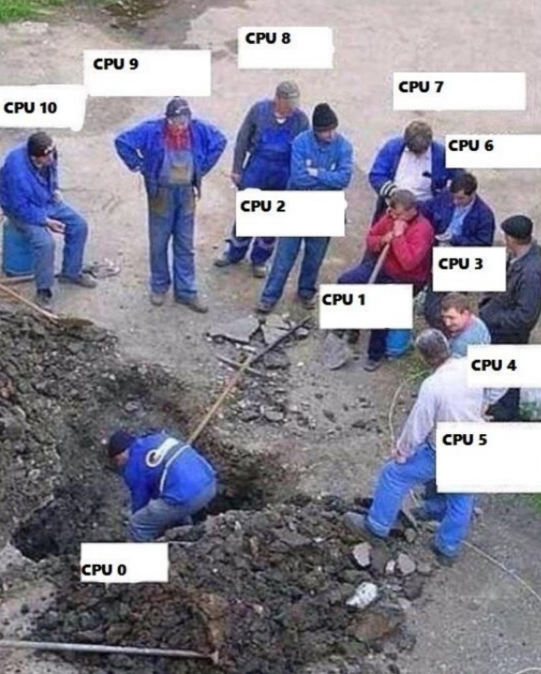
\includegraphics[width=0.9\columnwidth]{images/python_concurrency.png}
   \label{fig:python_concurrency}
\end{figure}
\end{paracol}

\subsubsection{Alternatives}
It is believed that overcoming the GIL performance issue would make the
implementation much more complicated and therefore costlier to \textit{maintain}.
\textbf{Jython} and \textbf{IronPython} have no GIT and fully exploit multiprocessor architecture capabilities.
In Cython the GIL may be released temporarily using the \lstinline|with| statement.

\section{Criticism}
Tuples are made by the commas, not by \lstinline|( )| with the exception of the empty tuple…
\begin{lstlisting}
   >>> type((1,2,3))
   <class 'tuple'>
   >>> type(())
   <class 'tuple'>
   >>> type((1))
   <class 'int'>
   >>> type((1,))
   <class 'tuple'>
\end{lstlisting}

\textbf{Lack of brackets} makes the syntax \textit{"weaker"} than
in other languages:
accidental changes of
indentation may change the semantics, leaving
the program syntactically correct.
\begin{center}
\textit{\underline{Will Python change on this matter?}}
\end{center}
\begin{lstlisting}
   >>> from __future__ import braces
      File "<stdin>", line 1
   SyntaxError: not a chance
\end{lstlisting}